\input{../../input/main}

\begin{document}

\begin{center}
  \Large{\textbf{Городской центр физического образования, 10 класс.}\\
  \textit{Серия 13, 15 января 2015.}}
\end{center}

\begin{center}
  \Large\textbf{ Для общего образования. }
\end{center}

\large

\task{ В шесть рёбер куба впаяны одинаковые резисторы с
  сопротивлениями $R$. Сопротивления перемычек в остальных ребрах
  одинаковы и очень малы. Источник напряжения $U$ подключен к выводам
  1 и 3 куба. Найдите токи, текущие через рёбра куба, и общее
  сопротивление куба.}
\begin{center}
  \begin{tikzpicture}[circuit ee IEC,thick]
    \node[contact] (1) at (0,0) {};
    \node[contact] (2) at (2,2) {};
    \node[contact] (3) at (5,2) {};
    \node[contact] (4) at (3,0) {};
    \node[contact] (5) at (0,3) {};
    \node[contact] (6) at (2,5) {};
    \node[contact] (7) at (5,5) {};
    \node[contact] (8) at (3,3) {}; 
    \draw (1) node[below] {1} to[resistor] (2) node[above left] {2} to
    [resistor] (3) node[right] {3} to[resistor] (4) node[below] {4} --
    (1);
    \draw (5) node[left] {5} to[resistor] (6) node[above left] {6} --
    (7) node[right] {7} to[resistor] (8) node[right] {8} --
    (5);
    \draw (1) -- (5);
    \draw (2) to[resistor] (6);
    \draw (4) -- (8);
    \draw (3) -- (7); 
  \end{tikzpicture}
\end{center}

\task{ Вася нашел старую медную проволоку с сильно попорченной
  изоляцией. Намереваясь сдать в пункт приема цветных металлов медь,
  он скомкал проволоку и бросил комок в костер. После такой обработки
  полностью избавленная от изоляции медь массой 2 кг имела температуру
  $600^{\circ}$C. Вася зацепил проволоку железным крючком и, не
  торопясь, опустил горячий комок проволоки в открытое ведро с 5
  литрами воды при начальной температуре $20^{\circ}$C. Когда
  перестало раздаваться шипение, Вася круговыми движениями комка
  проволоки перемешал воду в ведре. Какой стала температура воды в
  ведре после того, как медь остыла? Удельная теплоемкость меди равна
  примерно $380 \mbox{ Дж/кг}\cdot{}^{\circ}$C, удельная теплоемкость воды
  $4200 \mbox{ Дж/кг}\cdot {}^{\circ}$C, удельная теплота испарения воды 2,3
  МДж/кг. }

\task{ Два маленьких шарика 1 и 2, масса каждого из которых $m$,
  соединены невесомым стержнем длиной $L$. Первый шарик шарнирно
  закреплён в точке \textbf{O}, а второй шарик совершает колебания в
  вертикальной плоскости. В один из моментов, когда стержень был
  вертикален, верхний шарик освободили из крепления. Когда угол между
  стержнем и вертикалью оказался равным $\beta>0$, шарик 2 приблизился
  к прямой \textbf{AB} на минимальное расстояние. С какой скоростью
  двигался шарик 2 в момент освобождения шарика 1? Сопротивлением
  воздуха пренебречь. }
\begin{center}
  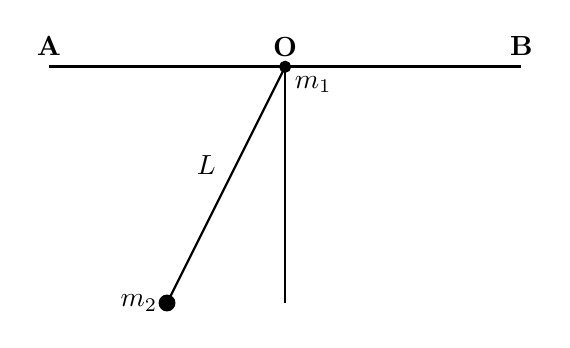
\begin{tikzpicture}
    \draw[very thick] (0,0) node[above] {\textbf{A}} -- (6,0)
    node[above] {\textbf{B}};
    \draw[fill=black] (3,0) circle (0.07cm) node[above] {\textbf{O}}
    node[below right] {$m_1$};
    \draw[thick] (3,0) -- (3,-3);
    \draw[thick] (3,0) -- (1.5,-3) node[midway,above left] {$L$};
    \draw[fill=black] (1.5,-3) circle (0.1cm) node[left] {$m_2$}; 
  \end{tikzpicture}
\end{center}

\task{ На горизонтальном столе находятся два одинаковых грузика,
  связанные невесомой и нерастяжимой нитью, образующей равнобедренный
  треугольник \textbf{AOB}. Углы при основаниях треугольника равны
  $\alpha$. В точке \textbf{O} к этой нити привязана другая нить,
  которую удерживают вертикально слегка натянутой. С каким минимальным
  ускорением нужно начать поднимать точку \textbf{O}, чтобы грузы оторвались от
  стола в момент начала своего движения? }
\begin{center}
  \begin{tikzpicture}
    \draw[thick,interface] (6,0) -- (0,0);
    \draw[thick,fill=gray!20] (1,0) rectangle (1.8,0.75);
    \draw[thick,fill=gray!20] (5,0) rectangle ++(-0.8,0.75);
    \draw[thick] (1.4,0.75) node[above left] {\textbf{A}} -- (3,2)
    node[below] {\textbf{O}} -- (4.6,0.75) node[above right] {\textbf{B}};
    \draw[thick] (3,2) -- (3,3);
    \draw[thick,dashed] (1.4,0.75) -- (4.6,0.75); 
  \end{tikzpicture}
\end{center}

\end{document}


%%% Local Variables: 
%%% mode: latex
%%% TeX-engine:xetex
%%% TeX-PDF-mode: t
%%% End:
